
\subsection{MULTI-RESOLUTION MATCH CRITERIA}
Method to track object at image is based on PIV. Figure 2(a) shows the application 
in 2 dimensions and the next in
3 dimensions.

\begin{figure}[H]
\centering
  \subfloat[]{\label{subfig:(a)} 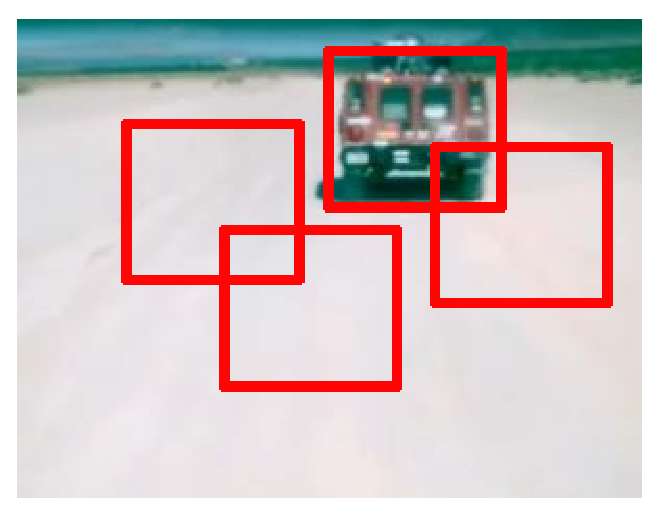
\includegraphics[width=.5\columnwidth]{images/figure2a.eps}}
  \subfloat[]{\label{subfig:(b)} 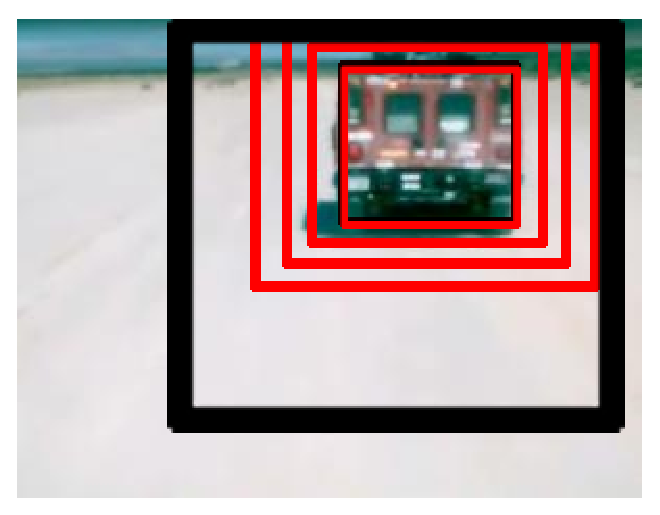
\includegraphics[width=.5\columnwidth]{images/figure2b.eps}}
  \caption{The red box in figure (a) shows the ROI and black box is WOS. In the figure (a), 
  ROI is compared with first portion on the left top of WOS, and these comparisons are made 
  pixel by pixel for whole WOS. The black boxes, in the figure (b), are the WOS used 
  to different layers of search in 3 dimensions}
\end{figure}

To track the object, the ROI defines the size of WOS and, verify the similarity 
of ROI and parts of WOS using PCC. 
The highest coefficient of Pearson determines new place of object. The figure 2(b) 
reveals how the dimension of depth was included and, 
the search is made in different layers. In 3 dimensions, the target also is found 
from the highest PCC among WOS, but the object may be 
bigger or smaller, depending in which layers was.\\
%onde estava, onde esta agora
%que tamanho tinha que tamanho tem.